\chapter{Experiments and Results}

In this chapter, we present experiments we did in this work and some valuable results we have achieved. We did experiments in both synthetic data and real data. We started with synthetic data to check how well our model can predict camera location in synthetic data on exactly same objects. It turns out the network can predict quite accurately for synthetic data. Then we did experiments in real data. We hope that by mixing synthetic data together with real data as training data, we can improve the result of prediction in real data.

\section{Synthetic Data}

We first did experiments on multiple views of a single object generated by SIXD Toolkit. We use objects from SunCG, and we generate multiple views of the object in random texture, with random translation within the camera's field of view, and with random distance to the object. We are also training with data in random background, testing in both no background and random background. As a result, the prediction is very accurate. Taking a 5 px threshold, the accuracy that the error of 2D projection of all vertices of the object 3D mesh between prediction and ground truth within the threshold is greater than 70\%. Figure \ref{fig:sixd} shows the predictions on the test data of our generated synthetic data with no background. The red bounding box is the ground truth, the yellow box is the predicted 2D locations of the projected bounding box, the blue box is the reprojected bounding box using the camera pose computed from ground truth 2D locations i.e. the red box corners and given 3D control points locations, and finally the green box is the reprojected box using the camera pose computed from predicted 2D locations i.e. the yellow box corners and given 3D control points locations.

\begin{figure}[h!]
  \centering
  \begin{subfigure}[b]{0.32\linewidth}
    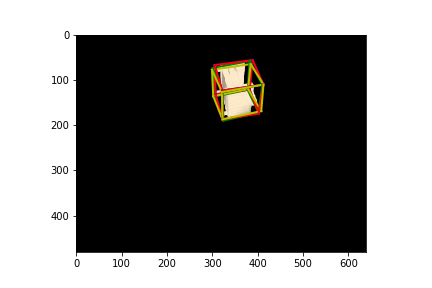
\includegraphics[width=\linewidth]{results/sixd/0267.png}
  \end{subfigure}
  \begin{subfigure}[b]{0.32\linewidth}
    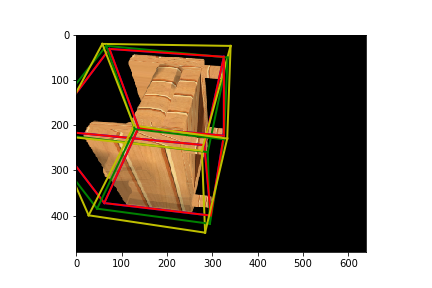
\includegraphics[width=\linewidth]{results/sixd/0298.png}
  \end{subfigure}
  \begin{subfigure}[b]{0.32\linewidth}
    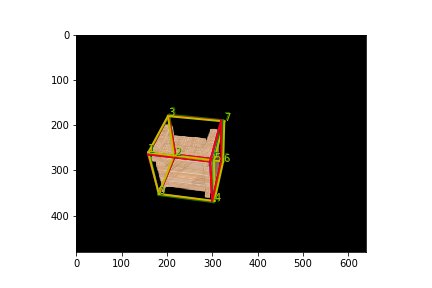
\includegraphics[width=\linewidth]{results/sixd/0501.png}
  \end{subfigure}
  \begin{subfigure}[b]{0.32\linewidth}
    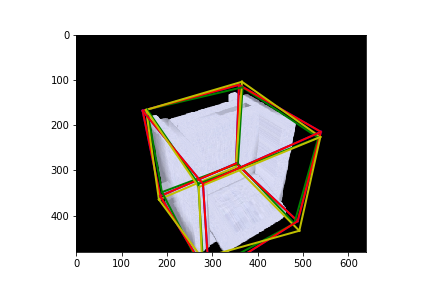
\includegraphics[width=\linewidth]{results/sixd/0529.png}
  \end{subfigure}
  \begin{subfigure}[b]{0.32\linewidth}
    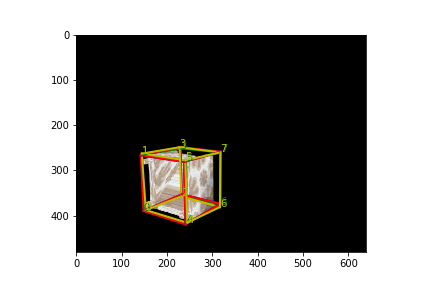
\includegraphics[width=\linewidth]{results/sixd/1151.png}
  \end{subfigure}
  \begin{subfigure}[b]{0.32\linewidth}
    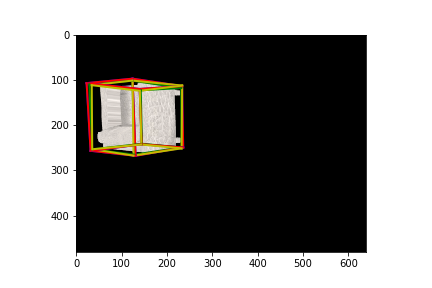
\includegraphics[width=\linewidth]{results/sixd/1186.png}
  \end{subfigure}
  \caption{Examples of results of sofa object in multiple views generated with SIXD Tookit}
  \label{fig:sixd}
\end{figure}

Then we did experiments on the whole synthetic image. We use SunCG toolbox to render the whole synthetic indoor environment images provided in SunCG dataset. Specifically, we filter out scenes containing our target object - sofa, render images of the scenes, and filter out images containing the object with the rules we stated in section \ref{sec:data_filtering}. Figure \ref{fig:suncg} shows the results of testing on SunCG dataset.

\begin{figure}[h!]
  \centering
  \begin{subfigure}[b]{0.32\linewidth}
    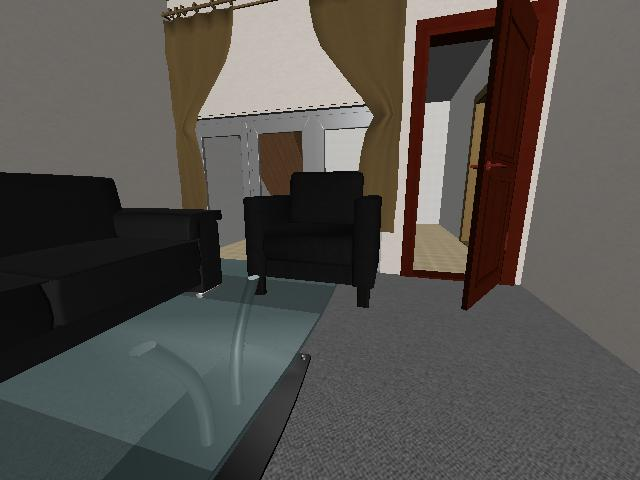
\includegraphics[width=\linewidth]{results/suncg/000004_color.jpg}
  \end{subfigure}
  \begin{subfigure}[b]{0.32\linewidth}
    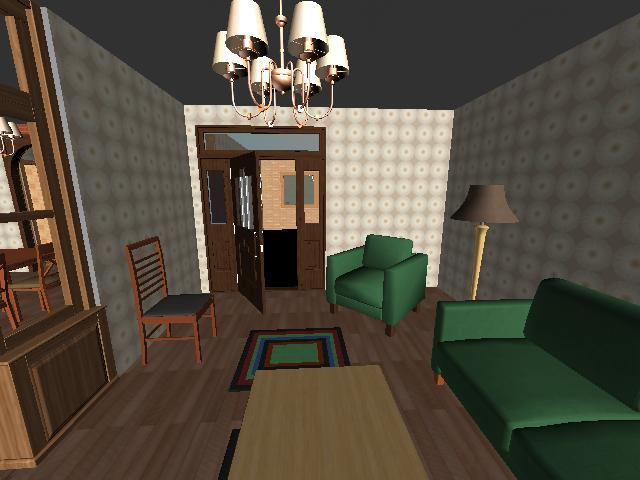
\includegraphics[width=\linewidth]{results/suncg/000005_color.jpg}
  \end{subfigure}
  \begin{subfigure}[b]{0.32\linewidth}
    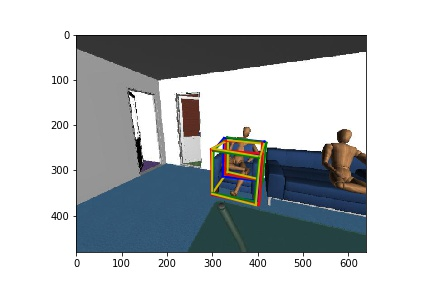
\includegraphics[width=\linewidth]{results/suncg/000006_color.jpg}
  \end{subfigure}
  \begin{subfigure}[b]{0.32\linewidth}
    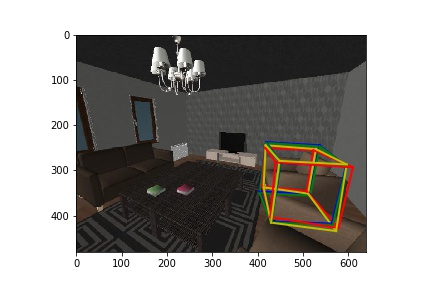
\includegraphics[width=\linewidth]{results/suncg/000007_color.jpg}
  \end{subfigure}
  \begin{subfigure}[b]{0.32\linewidth}
    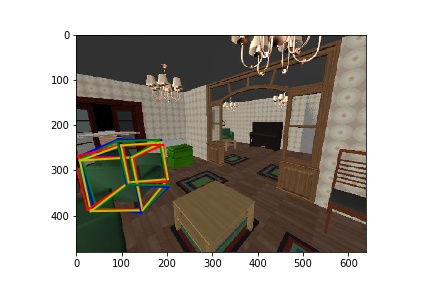
\includegraphics[width=\linewidth]{results/suncg/000017_color.jpg}
  \end{subfigure}
  \begin{subfigure}[b]{0.32\linewidth}
    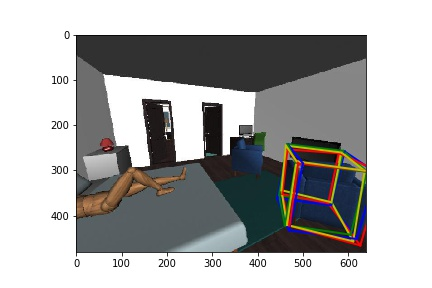
\includegraphics[width=\linewidth]{results/suncg/000020_color.jpg}
  \end{subfigure}
  \begin{subfigure}[b]{0.32\linewidth}
    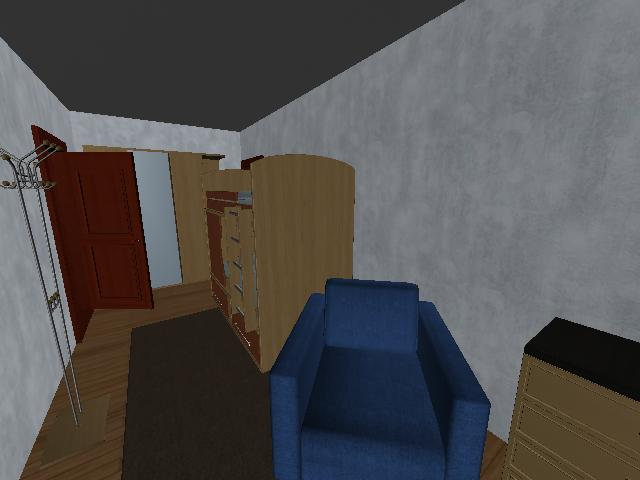
\includegraphics[width=\linewidth]{results/suncg/000031_color.jpg}
  \end{subfigure}
  \begin{subfigure}[b]{0.32\linewidth}
    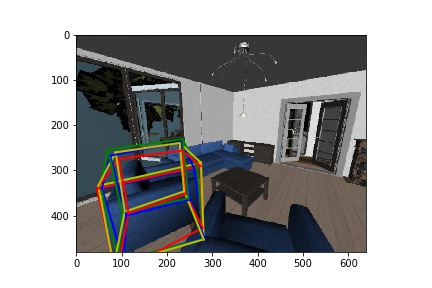
\includegraphics[width=\linewidth]{results/suncg/000034_color.jpg}
  \end{subfigure}
  \begin{subfigure}[b]{0.32\linewidth}
    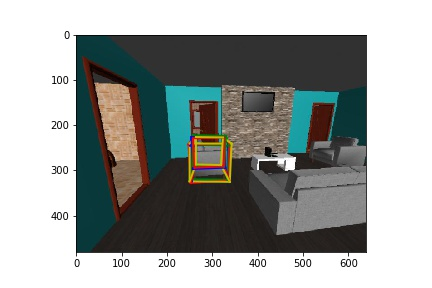
\includegraphics[width=\linewidth]{results/suncg/000045_color.jpg}
  \end{subfigure}
  \begin{subfigure}[b]{0.32\linewidth}
    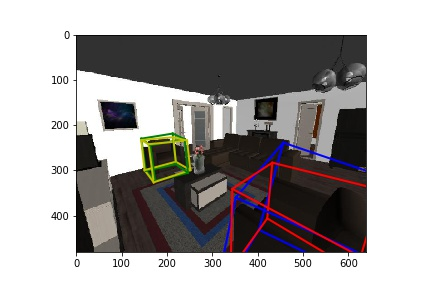
\includegraphics[width=\linewidth]{results/suncg/000050_color.jpg}
  \end{subfigure}
  \begin{subfigure}[b]{0.32\linewidth}
    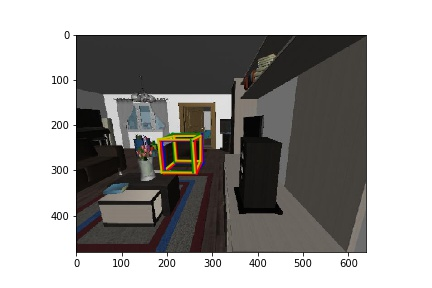
\includegraphics[width=\linewidth]{results/suncg/000055_color.jpg}
  \end{subfigure}
  \begin{subfigure}[b]{0.32\linewidth}
    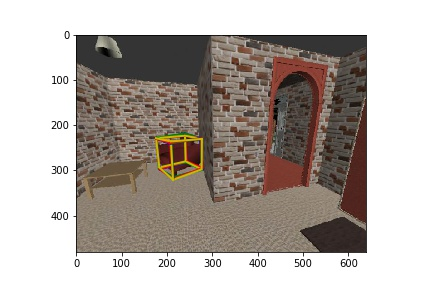
\includegraphics[width=\linewidth]{results/suncg/000057_color.jpg}
  \end{subfigure}
  \begin{subfigure}[b]{0.32\linewidth}
    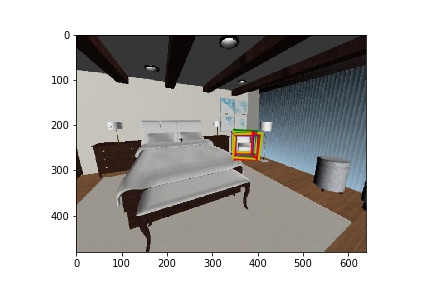
\includegraphics[width=\linewidth]{results/suncg/000058_color.jpg}
  \end{subfigure}
  \begin{subfigure}[b]{0.32\linewidth}
    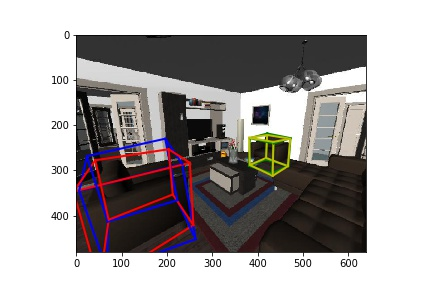
\includegraphics[width=\linewidth]{results/suncg/000060_color.jpg}
  \end{subfigure}
  \begin{subfigure}[b]{0.32\linewidth}
    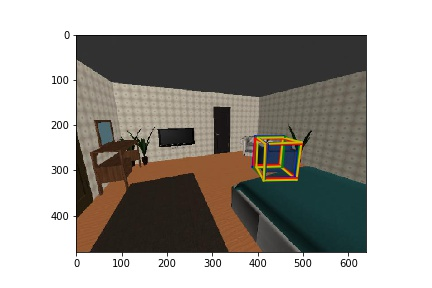
\includegraphics[width=\linewidth]{results/suncg/000061_color.jpg}
  \end{subfigure}
  \begin{subfigure}[b]{0.32\linewidth}
    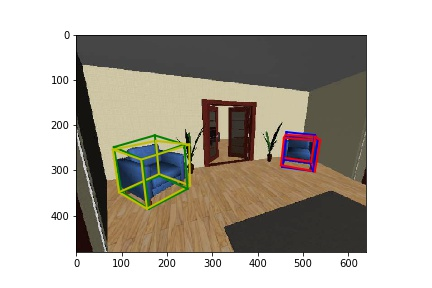
\includegraphics[width=\linewidth]{results/suncg/000066_color.jpg}
  \end{subfigure}
  \begin{subfigure}[b]{0.32\linewidth}
    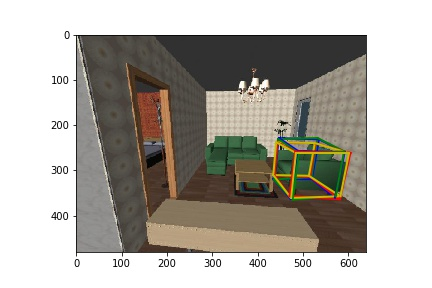
\includegraphics[width=\linewidth]{results/suncg/000073_color.jpg}
  \end{subfigure}
  \begin{subfigure}[b]{0.32\linewidth}
    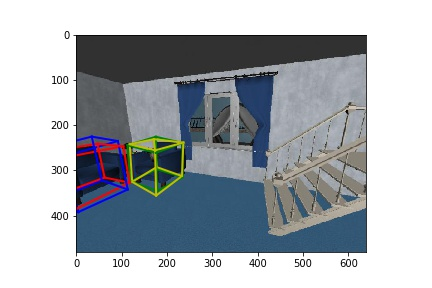
\includegraphics[width=\linewidth]{results/suncg/000096_color.jpg}
  \end{subfigure}
  \caption{Examples of results of sofa object in SunCG test dataset}
  \label{fig:suncg}
\end{figure}

\section{Real Data}

For real data, we still have a lot of space for improvement. We will explain in more details in next chapter. However, we already achieve some good results on real data for single object camera pose detection. We get our training and testing data from 264 different scenes and in total 565 scans. Here are some results on Scannet Dataset.

Our model performs very well on training data or data from the same scene. When test on new scenes, which the network has never seen in the training period, we also get some quite good predictions. Figure \ref{fig:result_couch} shows some examples of the good results we get on couch object in ScanNet test scenes. The red bounding boxes are the ground truth and the yellow bounding  boxes are the predicted 2D points locations. As we can see, our model is robust to occlusion and different sizes of the object. Sometimes our ground truth label is not accurate due to the reasons we have explained in last chapter, and the predictions can even fix the noise and make a better bounding box than our labels. For example our ground truth label may not be upright due to noises in camera pose or incomplete construction of the object model, and the predicted bounding box can be upright and fit the object better.

\begin{figure}[h!]
  \centering
  \begin{subfigure}[b]{0.32\linewidth}
    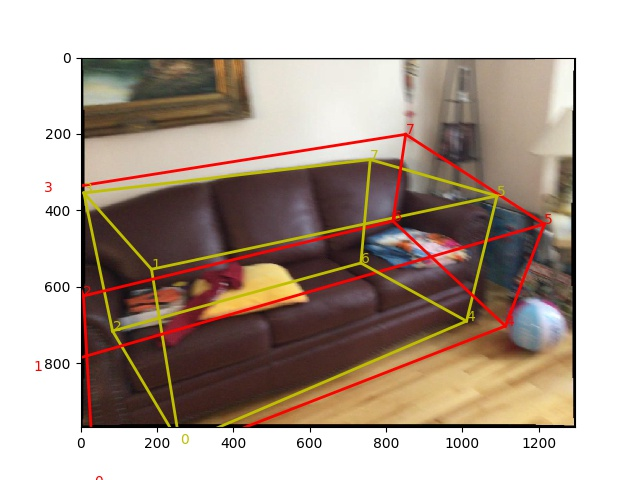
\includegraphics[width=\linewidth]{results/couch/scene0024_02_2776.jpg}
  \end{subfigure}
  \begin{subfigure}[b]{0.32\linewidth}
    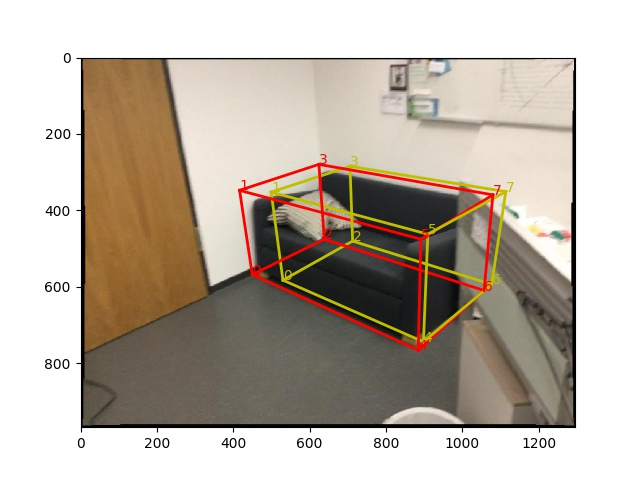
\includegraphics[width=\linewidth]{results/couch/scene0025_00_516.jpg}
  \end{subfigure}
  \begin{subfigure}[b]{0.32\linewidth}
    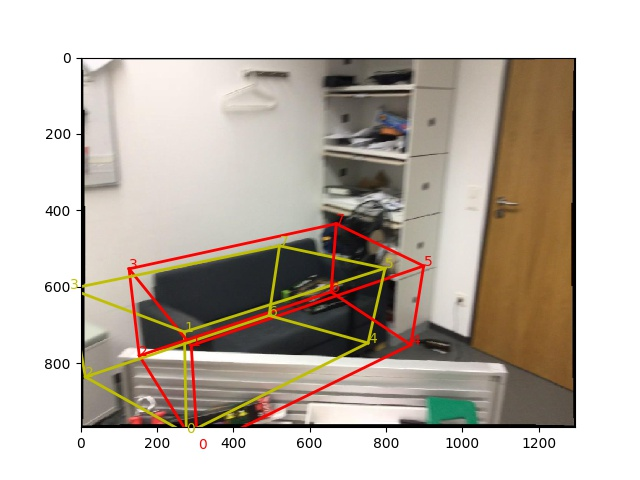
\includegraphics[width=\linewidth]{results/couch/scene0025_01_516.jpg}
  \end{subfigure}
  \begin{subfigure}[b]{0.32\linewidth}
    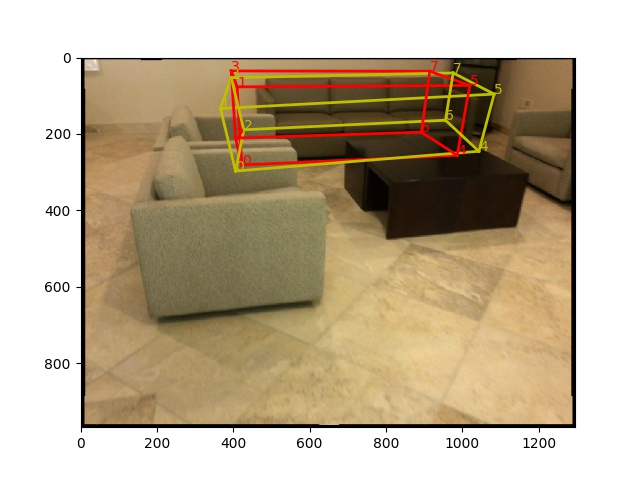
\includegraphics[width=\linewidth]{results/couch/scene0199_00_762.jpg}
  \end{subfigure}
  \begin{subfigure}[b]{0.32\linewidth}
    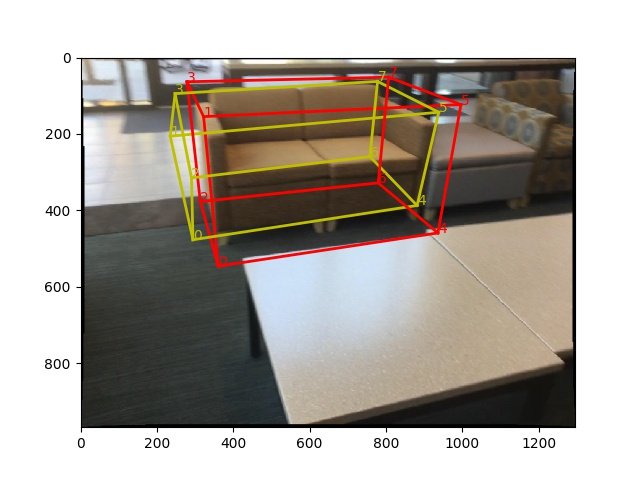
\includegraphics[width=\linewidth]{results/couch/scene0031_00_877.jpg}
  \end{subfigure}
  \begin{subfigure}[b]{0.32\linewidth}
    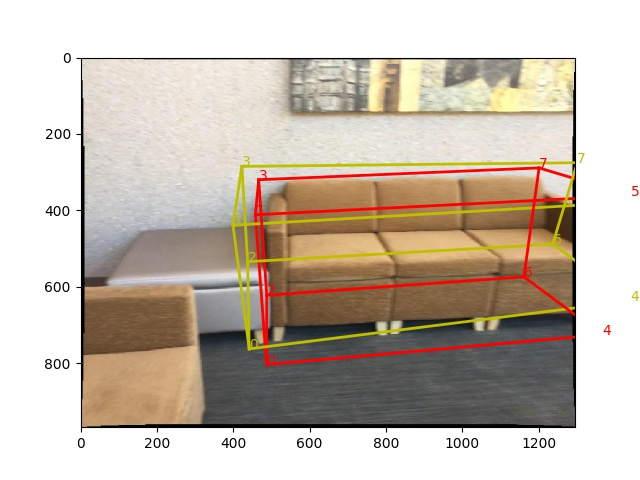
\includegraphics[width=\linewidth]{results/couch/scene0031_00_1644.jpg}
  \end{subfigure}
  \begin{subfigure}[b]{0.32\linewidth}
    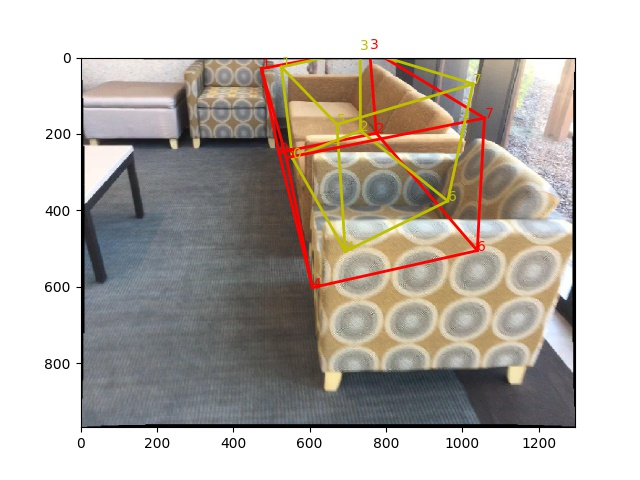
\includegraphics[width=\linewidth]{results/couch/scene0031_00_1900.jpg}
  \end{subfigure}
  \begin{subfigure}[b]{0.32\linewidth}
    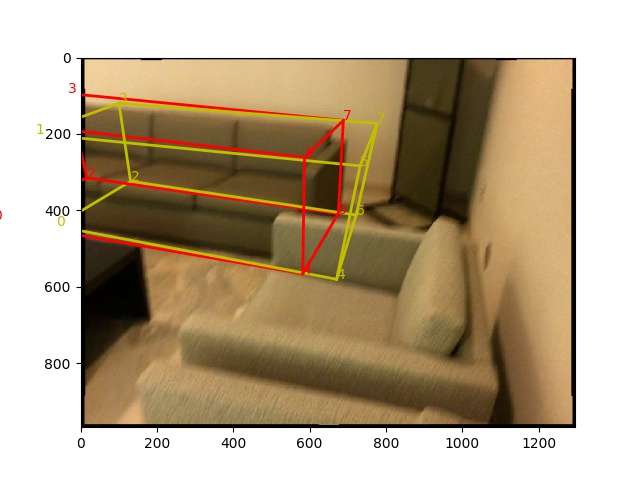
\includegraphics[width=\linewidth]{results/couch/scene0199_00_1471.jpg}
  \end{subfigure}
  \begin{subfigure}[b]{0.32\linewidth}
    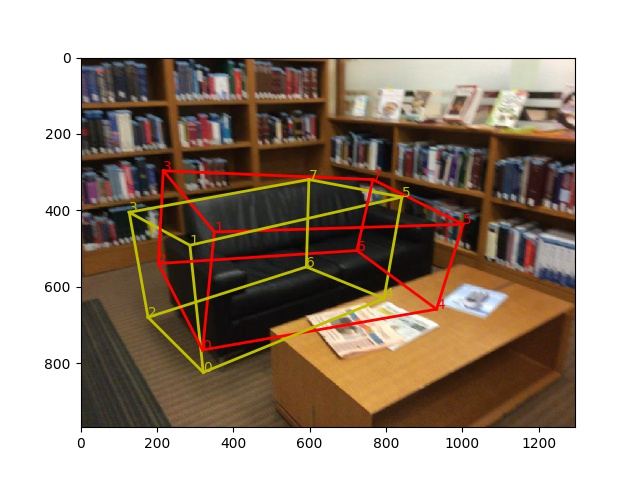
\includegraphics[width=\linewidth]{results/couch/scene0064_00_80.jpg}
  \end{subfigure}
  \begin{subfigure}[b]{0.32\linewidth}
    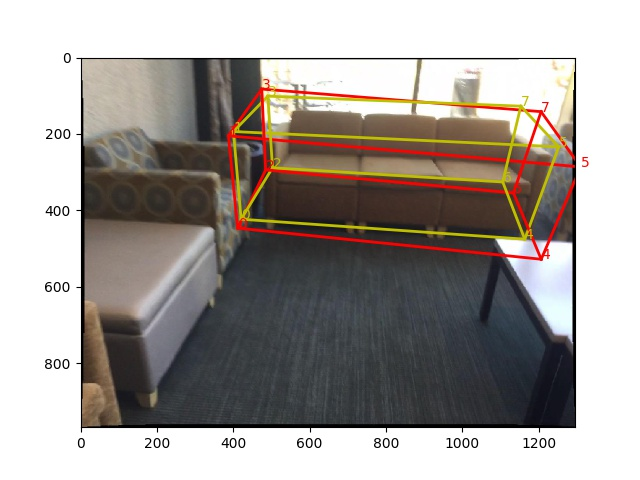
\includegraphics[width=\linewidth]{results/couch/scene0031_01_565.jpg}
  \end{subfigure}
  \begin{subfigure}[b]{0.32\linewidth}
    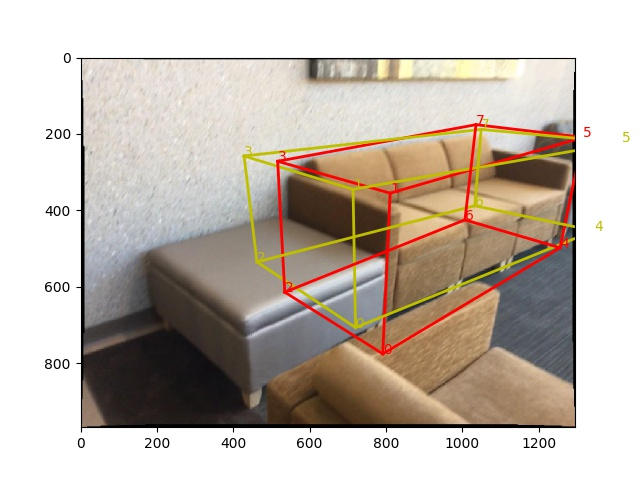
\includegraphics[width=\linewidth]{results/couch/scene0031_01_2147.jpg}
  \end{subfigure}
  \begin{subfigure}[b]{0.32\linewidth}
    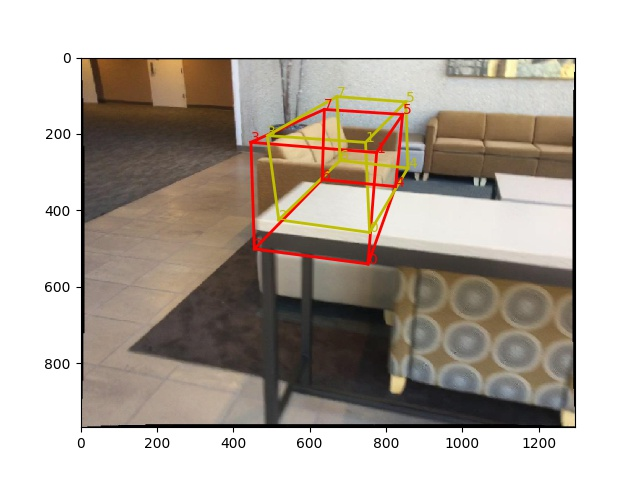
\includegraphics[width=\linewidth]{results/couch/scene0031_02_1702.jpg}
  \end{subfigure}
  \begin{subfigure}[b]{0.32\linewidth}
    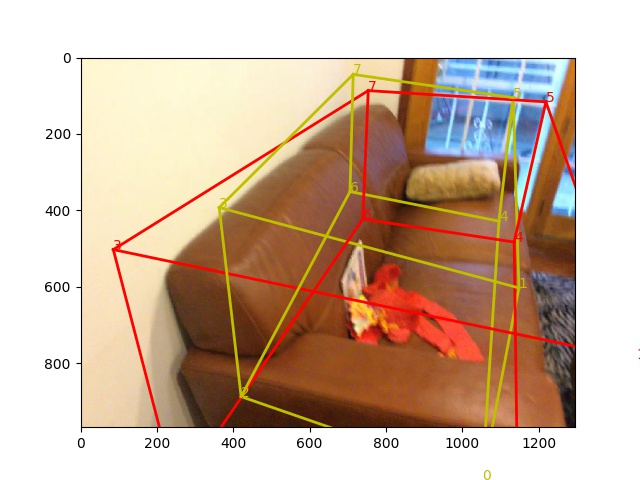
\includegraphics[width=\linewidth]{results/couch/scene0050_02_4364.jpg}
  \end{subfigure}
  \begin{subfigure}[b]{0.32\linewidth}
    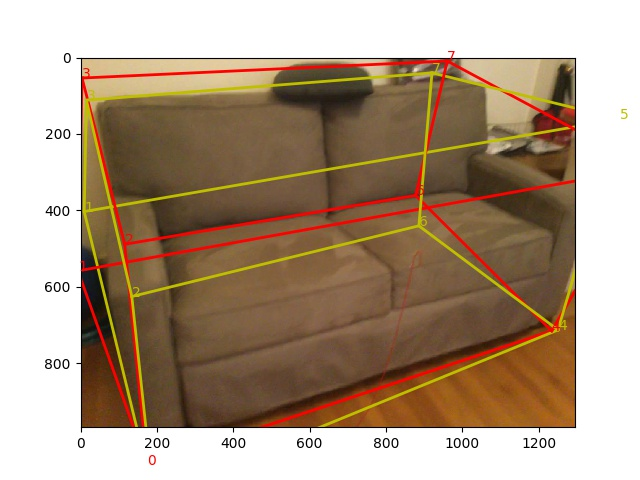
\includegraphics[width=\linewidth]{results/couch/scene0054_00_1691.jpg}
  \end{subfigure}
  \begin{subfigure}[b]{0.32\linewidth}
    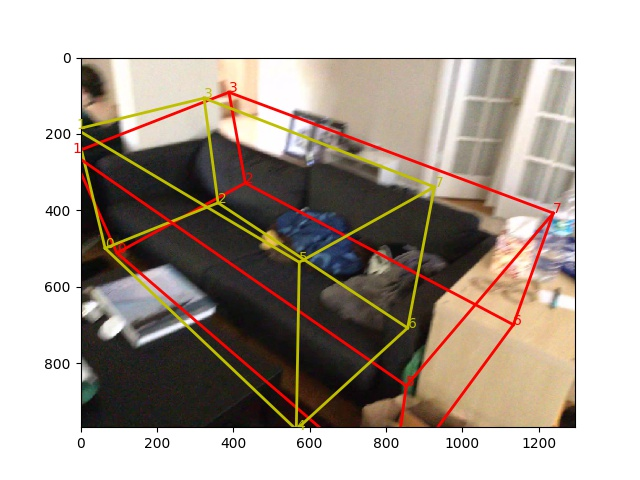
\includegraphics[width=\linewidth]{results/couch/scene0203_02_319.jpg}
  \end{subfigure}
  \caption{Examples of some good results of couch object in ScanNet test scenes}
  \label{fig:result_couch}
\end{figure}

Figure \ref{fig:result_couch_gt_err} shows some examples on different predictions with the ground truth, but they are not wrong. In this experiment, we try to filter out those images containing multiple same category objects. However, there are some noises maintain due to incomplete construction or objects in different sizes. As we mentioned before, we filter out those non-similar object model according to the difference of the size of its bounding box with our chosen 3D model. And when we choose images containing single target category object, we check that weather there are any other objects in the same category after filtering out similar objects. This means there may still be some other objects in the same category maintain in the image but with a different size i.e. out of the range of the threshold we set for bounding box size difference. Thus, when we test on these images, there may be other object predicted instead of the labeled one. As we can see, these predictions are not false, and should not contribute to our error measurements. Some of them predicts the other object in the image in the same category. Some of them try to fit in with a quite different shape which they have never seen during training period. And some of them may detected another category object but the appearance is very similar to our target object, which are sometimes even hard to distinguish for human beings. For example sometimes the network regards the pillow on the couch as the back of another small couch, which are quite reasonable predictions.

\begin{figure}[h!]
  \centering
  \begin{subfigure}[b]{0.32\linewidth}
    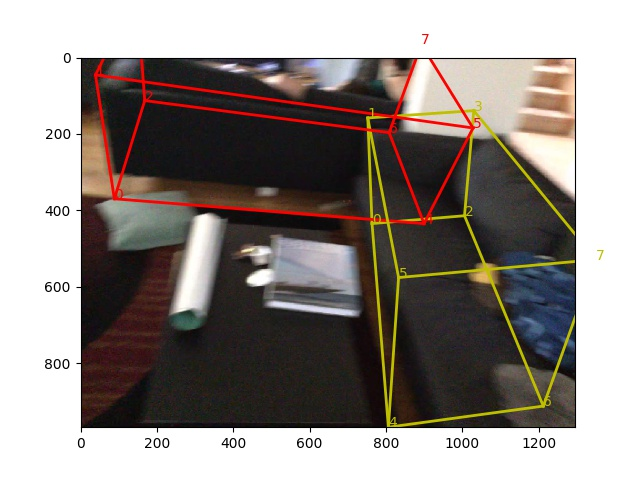
\includegraphics[width=\linewidth]{results/couch_gt_err/scene0203_02_941.jpg}
  \end{subfigure}
  \begin{subfigure}[b]{0.32\linewidth}
    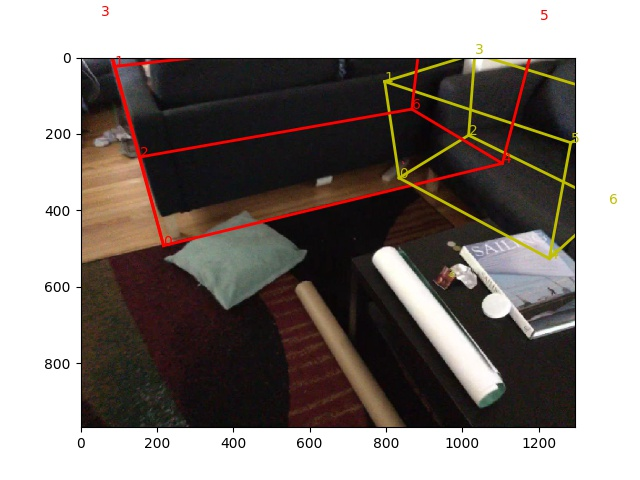
\includegraphics[width=\linewidth]{results/couch_gt_err/scene0203_01_774.jpg}
  \end{subfigure}
  \begin{subfigure}[b]{0.32\linewidth}
    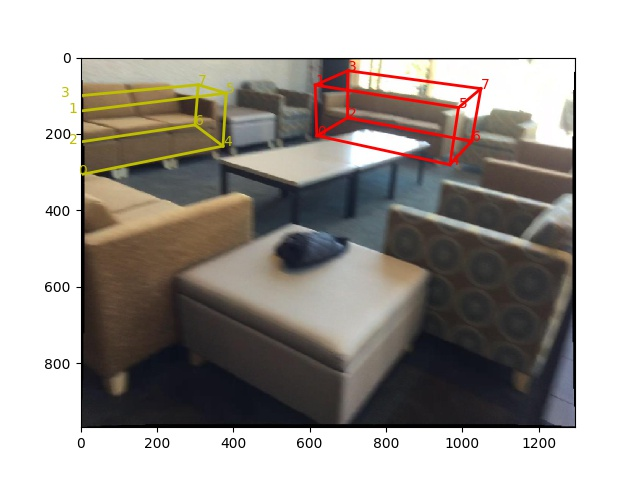
\includegraphics[width=\linewidth]{results/couch_gt_err/scene0031_00_2361.jpg}
  \end{subfigure}
  \begin{subfigure}[b]{0.32\linewidth}
    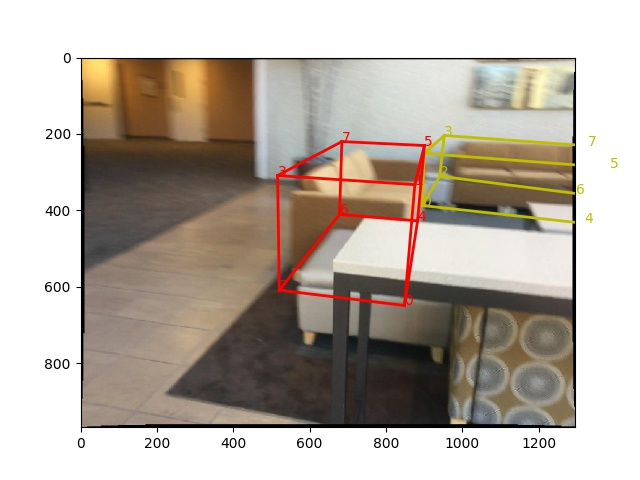
\includegraphics[width=\linewidth]{results/couch_gt_err/scene0031_01_1938.jpg}
  \end{subfigure}
  \begin{subfigure}[b]{0.32\linewidth}
    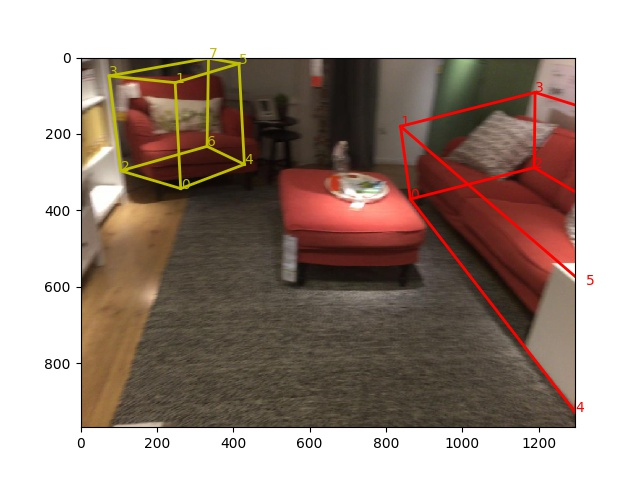
\includegraphics[width=\linewidth]{results/couch_gt_err/scene0049_00_192.jpg}
  \end{subfigure}
  \begin{subfigure}[b]{0.32\linewidth}
    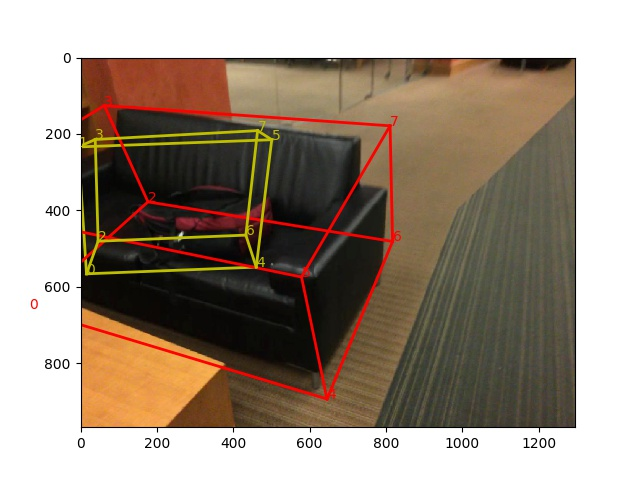
\includegraphics[width=\linewidth]{results/couch_gt_err/scene0064_00_319.jpg}
  \end{subfigure}
  \begin{subfigure}[b]{0.32\linewidth}
    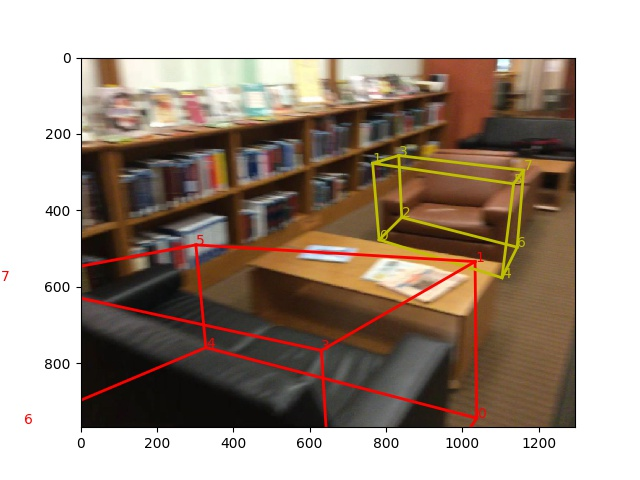
\includegraphics[width=\linewidth]{results/couch_gt_err/scene0064_00_1022.jpg}
  \end{subfigure}
  \begin{subfigure}[b]{0.32\linewidth}
    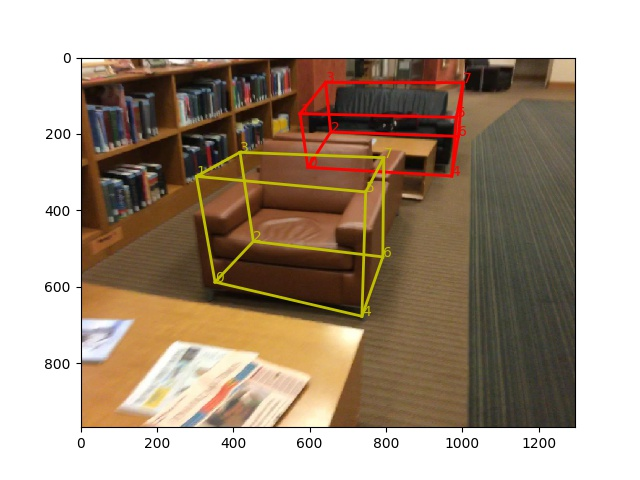
\includegraphics[width=\linewidth]{results/couch_gt_err/scene0064_00_1090.jpg}
  \end{subfigure}
  \begin{subfigure}[b]{0.32\linewidth}
    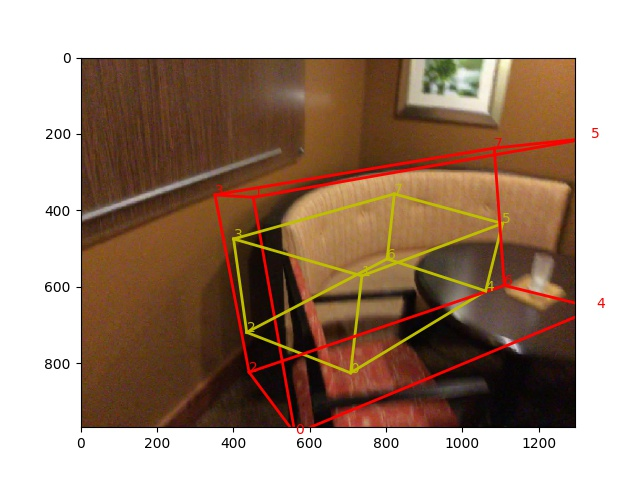
\includegraphics[width=\linewidth]{results/couch_gt_err/scene0132_00_1133.jpg}
  \end{subfigure}
  \begin{subfigure}[b]{0.32\linewidth}
    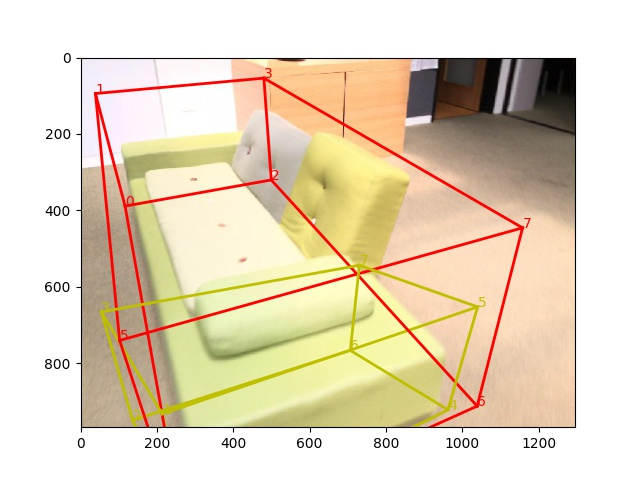
\includegraphics[width=\linewidth]{results/couch_gt_err/scene0148_00_1090.jpg}
  \end{subfigure}
  \begin{subfigure}[b]{0.32\linewidth}
    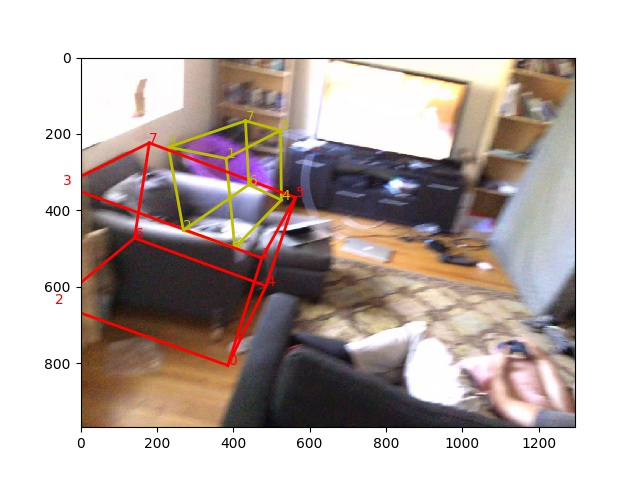
\includegraphics[width=\linewidth]{results/couch_gt_err/scene0203_02_1938.jpg}
  \end{subfigure}
  \begin{subfigure}[b]{0.32\linewidth}
    \includegraphics[width=\linewidth]{results/couch_gt_err/scene0031_02_2420.jpg}
  \end{subfigure}
  \caption{Examples of some reasonable results we of couch object in ScanNet test scenes}
  \label{fig:result_couch_gt_err}
\end{figure}

There are also a lot of failed cases. Figure \ref{fig:result_couch_err} shows these incorrect predictions. Consider the reasoning, there are less accuracy for predictions from the back of the couch. This is also reasonable for human beings, as it's a lack of important features when only the back of the couch is present in the image. The predictions are poorer for the objects having similar texture or color with the background, which is sometimes also difficult to distinguish in human eyes. The predictions are also poorer for the object containing different textures or colors itself. This may make the network partition the object and predict only part of the object. For example, the network has never seen a couch having different colors in its back, or couch with no back in some part, and the model only predict a part of the couch which contains  a back and consists of only one color/texture. And finally, those object in quite special shapes that the network has never seen during training result in poor predictions. Of course our training data size is not big enough. By enlarging the size of the training dataset, our model  may generalize better to more different shapes of the objects in the same category.

\begin{figure}[h!]
  \centering
  \begin{subfigure}[b]{0.32\linewidth}
    \includegraphics[width=\linewidth]{results/couch_err/scene0234_00_368.jpg}
  \end{subfigure}
  \begin{subfigure}[b]{0.32\linewidth}
    \includegraphics[width=\linewidth]{results/couch_err/scene0031_02_1860.jpg}
  \end{subfigure}
  \begin{subfigure}[b]{0.32\linewidth}
    \includegraphics[width=\linewidth]{results/couch_err/scene0050_01_993.jpg}
  \end{subfigure}
  \begin{subfigure}[b]{0.32\linewidth}
    \includegraphics[width=\linewidth]{results/couch_err/scene0064_00_981.jpg}
  \end{subfigure}
  \begin{subfigure}[b]{0.32\linewidth}
    \includegraphics[width=\linewidth]{results/couch_err/scene0141_02_618.jpg}
  \end{subfigure}
  \begin{subfigure}[b]{0.32\linewidth}
    \includegraphics[width=\linewidth]{results/couch_err/scene0148_00_565.jpg}
  \end{subfigure}
  \begin{subfigure}[b]{0.32\linewidth}
    \includegraphics[width=\linewidth]{results/couch_err/scene0148_00_893.jpg}
  \end{subfigure}
  \begin{subfigure}[b]{0.32\linewidth}
    \includegraphics[width=\linewidth]{results/couch_err/scene0203_00_503.jpg}
  \end{subfigure}
  \begin{subfigure}[b]{0.32\linewidth}
    \includegraphics[width=\linewidth]{results/couch_err/scene0203_00_608.jpg}
  \end{subfigure}
  \begin{subfigure}[b]{0.32\linewidth}
    \includegraphics[width=\linewidth]{results/couch_err/scene0203_00_1446.jpg}
  \end{subfigure}
  \begin{subfigure}[b]{0.32\linewidth}
    \includegraphics[width=\linewidth]{results/couch_err/scene0203_02_336.jpg}
  \end{subfigure}
  \begin{subfigure}[b]{0.32\linewidth}
    \includegraphics[width=\linewidth]{results/couch_err/scene0203_02_1991.jpg}
  \end{subfigure}
  \caption{Examples of some failed results of couch object in ScanNet test scenes}
  \label{fig:result_couch_err}
\end{figure}

\begin{figure}[h!]
  \centering
  \begin{subfigure}[b]{0.32\linewidth}
    \includegraphics[width=\linewidth]{results/chair/scene0005_01_1152.jpg}
  \end{subfigure}
  \begin{subfigure}[b]{0.32\linewidth}
    \includegraphics[width=\linewidth]{results/chair/scene0006_00_691.jpg}
  \end{subfigure}
  \begin{subfigure}[b]{0.32\linewidth}
    \includegraphics[width=\linewidth]{results/chair/scene0006_02_2664.jpg}
  \end{subfigure}
  \begin{subfigure}[b]{0.32\linewidth}
    \includegraphics[width=\linewidth]{results/chair/scene0030_00_336.jpg}
  \end{subfigure}
  \begin{subfigure}[b]{0.32\linewidth}
    \includegraphics[width=\linewidth]{results/chair/scene0030_02_364.jpg}
  \end{subfigure}
  \begin{subfigure}[b]{0.32\linewidth}
    \includegraphics[width=\linewidth]{results/chair/scene0041_01_243.jpg}
  \end{subfigure}
  \begin{subfigure}[b]{0.32\linewidth}
    \includegraphics[width=\linewidth]{results/chair/scene0045_01_1384.jpg}
  \end{subfigure}
  \begin{subfigure}[b]{0.32\linewidth}
    \includegraphics[width=\linewidth]{results/chair/scene0056_00_1932.jpg}
  \end{subfigure}
  \begin{subfigure}[b]{0.32\linewidth}
    \includegraphics[width=\linewidth]{results/chair/scene0127_00_516.jpg}
  \end{subfigure}
  \begin{subfigure}[b]{0.32\linewidth}
    \includegraphics[width=\linewidth]{results/chair/scene0131_01_762.jpg}
  \end{subfigure}
  \begin{subfigure}[b]{0.32\linewidth}
    \includegraphics[width=\linewidth]{results/chair/scene0131_01_877.jpg}
  \end{subfigure}
  \begin{subfigure}[b]{0.32\linewidth}
    \includegraphics[width=\linewidth]{results/chair/scene0138_00_119.jpg}
  \end{subfigure}
  \begin{subfigure}[b]{0.32\linewidth}
    \includegraphics[width=\linewidth]{results/chair/scene0163_00_2083.jpg}
  \end{subfigure}
  \begin{subfigure}[b]{0.32\linewidth}
    \includegraphics[width=\linewidth]{results/chair/scene0163_01_150.jpg}
  \end{subfigure}
  \begin{subfigure}[b]{0.32\linewidth}
    \includegraphics[width=\linewidth]{results/chair/scene0181_02_516.jpg}
  \end{subfigure}
  \begin{subfigure}[b]{0.32\linewidth}
    \includegraphics[width=\linewidth]{results/chair/scene0181_03_977.jpg}
  \end{subfigure}
  \begin{subfigure}[b]{0.32\linewidth}
    \includegraphics[width=\linewidth]{results/chair/scene0204_00_9.jpg}
  \end{subfigure}
  \begin{subfigure}[b]{0.32\linewidth}
    \includegraphics[width=\linewidth]{results/chair/scene0249_00_1127.jpg}
  \end{subfigure}
  \caption{Examples of the some good results of chair object in ScanNet test scenes}
  \label{fig:result_chair}
\end{figure}

\begin{figure}[h!]
  \centering
  \begin{subfigure}[b]{0.32\linewidth}
    \includegraphics[width=\linewidth]{results/table/scene0061_01_1531.jpg}
  \end{subfigure}
  \begin{subfigure}[b]{0.32\linewidth}
    \includegraphics[width=\linewidth]{results/table/scene0072_01_516.jpg}
  \end{subfigure}
  \begin{subfigure}[b]{0.32\linewidth}
    \includegraphics[width=\linewidth]{results/table/scene0125_00_45.jpg}
  \end{subfigure}
  \begin{subfigure}[b]{0.32\linewidth}
    \includegraphics[width=\linewidth]{results/table/scene0155_02_45.jpg}
  \end{subfigure}
  \begin{subfigure}[b]{0.32\linewidth}
    \includegraphics[width=\linewidth]{results/table/scene0196_00_1405.jpg}
  \end{subfigure}
  \begin{subfigure}[b]{0.32\linewidth}
    \includegraphics[width=\linewidth]{results/table/scene0244_00_319.jpg}
  \end{subfigure}
  \caption{Examples of the some good results of table object in ScanNet test scenes}
  \label{fig:result_table}
\end{figure}